% ============================================================================
\section{Résultats réels sur GCP}
\label{sec:reels}
% ============================================================================

\begin{center}
\fbox{\small Tous les chiffres de cette section sont des \textbf{mesures} sur les VM Google Cloud (\mesure{}).}
\end{center}

\subsection{Protocole}

Script \code{scripts/exp\_real.sh}. Pour chaque lot : le scheduler produit
l'allocation de RR et celle de \sel{} (avec leurs prédictions), puis
l'orchestrateur exécute chacune \textbf{3 fois, en alternance} (RR, \sel, RR,
\sel...) : une dérive des VM pendant la session touche ainsi les deux algorithmes.
Les 4 VM sont allumées (RR les utilise toutes) ; \sel{} n'envoie des tâches qu'aux
VM qu'il a choisies. Le coût mesuré applique la même règle que le modèle (fenêtre
active de chaque VM, minimum 60~s). Le score mesuré prend pour référence RR
\emph{mesuré} dans la même session.

Une \textbf{session} correspond à un démarrage des VM suivi de 3 exécutions
alternées par algorithme ; les VM sont arrêtées entre deux sessions. Les sessions
sont numérotées par lot. Comme la vitesse des VM change d'une session à l'autre
(section~\ref{sec:vm3}), les durées ne se comparent qu'à l'intérieur d'une même
session.

\paragraph{Un phénomène à garder en tête.} Pendant nos expériences, une VM
(vm3, une e2-medium) a régulièrement tourné jusqu'à deux fois moins vite que vm2,
de même type et avec la même charge. Nous parlons de VM \textbf{bridée}. Les
exécutions concernées sont signalées dans les tableaux, et la
section~\ref{sec:vm3} explique ce phénomène : c'est une particularité des VM à
cœur partagé de Google Cloud, pas un défaut de notre code.

\subsection{Synthèse : RR contre \sel{}}

\begin{table}[H]
\centering\small
\begin{tabular}{llrrrrrc}
\toprule
\textbf{Lot} & \textbf{Algorithme} & \textbf{Makespan (s)} & \textbf{Coût (\$)} & $\boldsymbol{D/\Drr}$ & $\boldsymbol{S}$ \textbf{mesuré} & $\boldsymbol{S}$ \textbf{prédit} & \textbf{VM} \\
\midrule
\multirow{2}{*}{9 tâches}    & RR    & 1,12 $\pm$ 0,09 & 0,004272 & 1,00 & 1,000 & 1,000 & 4 \\
                             & \sel  & 1,38 $\pm$ 0,15 & \textbf{0,001230} & 1,23 & \textbf{0,664} & 0,589 & 2 \\
\midrule
\multirow{2}{*}{500 tâches}  & RR    & 52,2 $\pm$ 19,2$^{*}$ & 0,004320 & 1,00 & 1,000 & 1,000 & 4 \\
                             & \sel  & 55,8 $\pm$ 16,9$^{*}$ & \textbf{0,003093} & 1,07 & \textbf{0,857} & 0,819 & 3 \\
\midrule
\multirow{2}{*}{2000 tâches} & RR    & 333,6 $\pm$ 6,7 & 0,011819 & 1,00 & 1,000 & 1,000 & 4 \\
                             & \sel  & \textbf{254,3 $\pm$ 2,8} & 0,011453 & 0,76 & \textbf{0,886} & 0,915 & 4 \\
\bottomrule
\end{tabular}
\caption{Moyenne $\pm$ écart-type sur 3 exécutions. Session~1 de chaque lot
(15/11, \code{results/exp\_real/}) ; vm3 était bridée pendant toutes les
exécutions de 2000 tâches. $D/\Drr$ : makespan mesuré divisé par celui de RR
mesuré, admissible si $\le 1{,}25$. $^{*}$ écart-type gonflé par le
ralentissement de vm3 (section~\ref{sec:vm3}).}
\label{tab:reels}
\end{table}

\begin{figure}[H]
\centering
\begin{tikzpicture}
\begin{axis}[
  ybar, width=0.36\textwidth, height=5.5cm, bar width=9pt,
  title={\small Coût mesuré (m\$)}, ymin=0, ymax=14,
  xtick={1,2,3}, xticklabels={9,500,2000}, xlabel={Tâches},
  xmin=0.5, xmax=3.5, grid=major, grid style={gray!20},
  legend style={font=\footnotesize, at={(0.03,0.97)}, anchor=north west}]
  \addplot[fill=rrcol] coordinates {(1,4.272) (2,4.320) (3,11.819)};
  \addplot[fill=selcol] coordinates {(1,1.230) (2,3.093) (3,11.453)};
  \legend{RR, \sel}
\end{axis}
\end{tikzpicture}\hfill
\begin{tikzpicture}
\begin{axis}[
  ybar, width=0.36\textwidth, height=5.5cm, bar width=9pt,
  title={\small Makespan mesuré (RR = 1)}, ymin=0.5, ymax=1.4,
  xtick={1,2,3}, xticklabels={9,500,2000}, xlabel={Tâches},
  xmin=0.5, xmax=3.5, grid=major, grid style={gray!20}]
  \addplot[fill=rrcol] coordinates {(1,1.000) (2,1.000) (3,1.000)};
  \addplot[fill=selcol] coordinates {(1,1.232) (2,1.069) (3,0.762)};
\end{axis}
\end{tikzpicture}\hfill
\begin{tikzpicture}
\begin{axis}[
  ybar, width=0.36\textwidth, height=5.5cm, bar width=9pt,
  title={\small Score $S$ mesuré}, ymin=0.5, ymax=1.1,
  xtick={1,2,3}, xticklabels={9,500,2000}, xlabel={Tâches},
  xmin=0.5, xmax=3.5, grid=major, grid style={gray!20}]
  \addplot[fill=rrcol] coordinates {(1,1.000) (2,1.000) (3,1.000)};
  \addplot[fill=selcol] coordinates {(1,0.664) (2,0.857) (3,0.886)};
\end{axis}
\end{tikzpicture}
\caption{RR contre \sel{} en conditions réelles (session~1) : coût,
makespan relatif à RR et score.}
\label{fig:reels}
\end{figure}

\paragraph{Lecture.}
\begin{itemize}
  \item \textbf{9 tâches} : 2 VM au lieu de 4, \textbf{coût $-71\,\%$}, mais
        lot 23\,\% plus long (modèle : $+4\,\%$), car 9 tâches sur 2 VM à
        2~vCPU ralentissent plus que prévu. La contrainte de délai est respectée
        de justesse ($D/\Drr = 1{,}23 \le 1{,}25$). Score : $-34\,\%$.
  \item \textbf{500 tâches} : vm1 éteinte, \textbf{coût $-29\,\%$}. Les $+7\,\%$
        de temps viennent d'une VM ralentie (section~\ref{sec:vm3}) : sans
        incident, les temps sont égaux (41,4 contre 41,5~s). Score : $-14\,\%$.
  \item \textbf{2000 tâches} : 4 VM mieux réparties, \textbf{temps $-24\,\%$},
        coût $-3\,\%$. Score : $-11\,\%$. Ce gain de temps est en partie dû au
        bridage de vm3 pendant cette session : RR lui confie 500 tâches, \sel{}
        seulement 398. Dans une autre session (tableau~\ref{tab:reels_tous}),
        le gain n'est que de 11\,\%.
\end{itemize}

\subsection{Comparaison réelle de tous les algorithmes}

Pour vérifier que \sel{} bat aussi les heuristiques classiques et pas seulement
Round Robin, nous avons exécuté tous les algorithmes sur GCP (même protocole :
3 exécutions alternées par algorithme ; \code{results/exp\_real\_all/}).

\begin{table}[H]
\centering\small
\begin{tabular}{lrrrrr}
\toprule
\textbf{Algorithme} & \textbf{Makespan mesuré (s)} & \textbf{Coût (\$)} & $\boldsymbol{D/\Drr}$ & $\boldsymbol{S}$ \textbf{mesuré} & $\boldsymbol{S}$ \textbf{prédit} \\
\midrule
\multicolumn{6}{l}{\textit{9 tâches (lot du TD3), session 2}} \\
\textbf{\sel}             & 1,20 $\pm$ 0,05 & \textbf{0,001230} & 0,92 & \textbf{0,541} & 0,589 \\
Allocation manuelle (TD3) & 1,25 $\pm$ 0,13 & 0,002458 & 0,96 & 0,731 & 0,745 \\
MET                       & 1,37 $\pm$ 0,04 & 0,002428 & 1,05 & 0,762 & 0,778 \\
Min-Min                   & 0,87 $\pm$ 0,03 & 0,004272 & 0,67 & 0,868 & 1,026 \\
Max-Min                   & 1,08 $\pm$ 0,07 & 0,004272 & 0,83 & 0,931 & 0,998 \\
MCT                       & 1,10 $\pm$ 0,06 & 0,004272 & 0,84 & 0,937 & 0,998 \\
Round Robin               & 1,30 $\pm$ 0,30 & 0,004272 & 1,00 & 1,000 & 1,000 \\
\midrule
\multicolumn{6}{l}{\textit{500 tâches, session 2}} \\
\textbf{\sel}             & 65,5 $\pm$ 9,3  & \textbf{0,003118} & 1,09 & \textbf{0,864} & 0,819 \\
Min-Min                   & 46,7 $\pm$ 12,2 & 0,004272 & 0,77 & 0,899 & 0,917 \\
Max-Min                   & 47,6 $\pm$ 9,0  & 0,004272 & 0,79 & 0,904 & 0,914 \\
MCT                       & 51,8 $\pm$ 17,0 & 0,004315 & 0,86 & 0,938 & 0,921 \\
Round Robin               & 60,3 $\pm$ 20,1 & 0,004353 & 1,00 & 1,000 & 1,000 \\
MET                       & 73,1 $\pm$ 18,6 & 0,003820 & 1,21 & 1,011 & 1,026 \\
\midrule
\multicolumn{6}{l}{\textit{2000 tâches, session 4$^{\ddagger}$}} \\
\textbf{\sel}             & 162,6 $\pm$ 2,6  & 0,007263 & 0,89 & \textbf{0,969} & 0,915 \\
MCT                       & 165,4 $\pm$ 1,2  & 0,007204 & 0,91 & 0,970 & 0,918 \\
Min-Min                   & 160,6 $\pm$ 3,1  & 0,007360 & 0,88 & 0,973 & 0,919 \\
Max-Min                   & 164,3 $\pm$ 2,1  & 0,007318 & 0,90 & 0,977 & 0,915 \\
Round Robin               & 182,4 $\pm$ 60,4 & \textbf{0,007117} & 1,00 & 1,000 & 1,000 \\
MET                       & 230,3 $\pm$ 14,5 & 0,008019 & \textbf{1,26}$^{\times}$ & 1,181 & 1,160 \\
\bottomrule
\end{tabular}
\caption{Tous les algorithmes exécutés sur GCP (\mesure{}), triés par score
mesuré. Chaque bloc vient d'une seule session, où tous les algorithmes ont été
exécutés en alternance : on compare les algorithmes à l'intérieur d'un bloc,
jamais d'un bloc à l'autre. Sessions du 16/11 (9 et 500 tâches le matin, 2000 tâches le soir),
\code{results/exp\_real\_all/}. $D/\Drr$ : makespan mesuré divisé par celui de
RR mesuré, admissible si $\le 1{,}25$ ; $^{\times}$ non admissible.
$^{\ddagger}$ VM démarrées sur processeur AMD EPYC 7B12, contre Intel Xeon @ 2.20GHz dans toutes les autres sessions (modèle relevé par l'orchestrateur).}
\label{tab:reels_tous}
\end{table}

\paragraph{Comparaison avec le tableau~\ref{tab:reels}.} Les deux tableaux
viennent d'exécutions faites à des moments différents, mais les scores de \sel{}
racontent la même chose : 0,664 puis 0,541 sur 9 tâches, 0,857 puis 0,864 sur
500 tâches, 0,886 puis 0,969 sur 2000 tâches. Il reste toujours sous 1, le score
de RR, et l'écart est le plus grand sur les petits lots, là où éteindre des VM
rapporte le plus.

\begin{figure}[H]
\centering
\begin{tikzpicture}
\begin{axis}[
  ybar, width=0.95\textwidth, height=6cm, bar width=6pt,
  ylabel={Score $S$ mesuré (plus bas = mieux)}, ymin=0.4, ymax=1.25,
  xtick={1,2,3}, xticklabels={9 tâches,500 tâches,2000 tâches}, xmin=0.5, xmax=3.5,
  grid=major, grid style={gray!20},
  legend style={at={(0.5,1.02)}, anchor=south, legend columns=4, font=\footnotesize},
  extra y ticks={1}, extra y tick style={grid style={black,dashed}}]
  \addplot[fill=rrcol]      coordinates {(1,1.000) (2,1.000) (3,1.000)};
  \addplot[fill=accent!60]  coordinates {(1,0.762) (2,1.011) (3,1.181)};
  \addplot[fill=gray!30]    coordinates {(1,0.937) (2,0.938) (3,0.970)};
  \addplot[fill=gray!55]    coordinates {(1,0.868) (2,0.899) (3,0.973)};
  \addplot[fill=gray!80]    coordinates {(1,0.931) (2,0.904) (3,0.977)};
  \addplot[fill=orange!60]  coordinates {(1,0.731) (2,0) (3,0)};
  \addplot[fill=selcol]     coordinates {(1,0.541) (2,0.864) (3,0.969)};
  \legend{RR, MET, MCT, Min-Min, Max-Min, Manuelle, \sel}
\end{axis}
\end{tikzpicture}
\caption{Score mesuré sur GCP. L'allocation manuelle n'existe que pour le lot de 9 tâches.}
\label{fig:reels_tous}
\end{figure}

\begin{figure}[H]
\centering
% Généré par ./bin/gantt à partir de : results/exp_real_all/tasks/rr_r1.csv results/exp_real_all/tasks/select-maxmin_r1.csv
% Durées MESURÉES par l'orchestrateur (start_s / end_s).
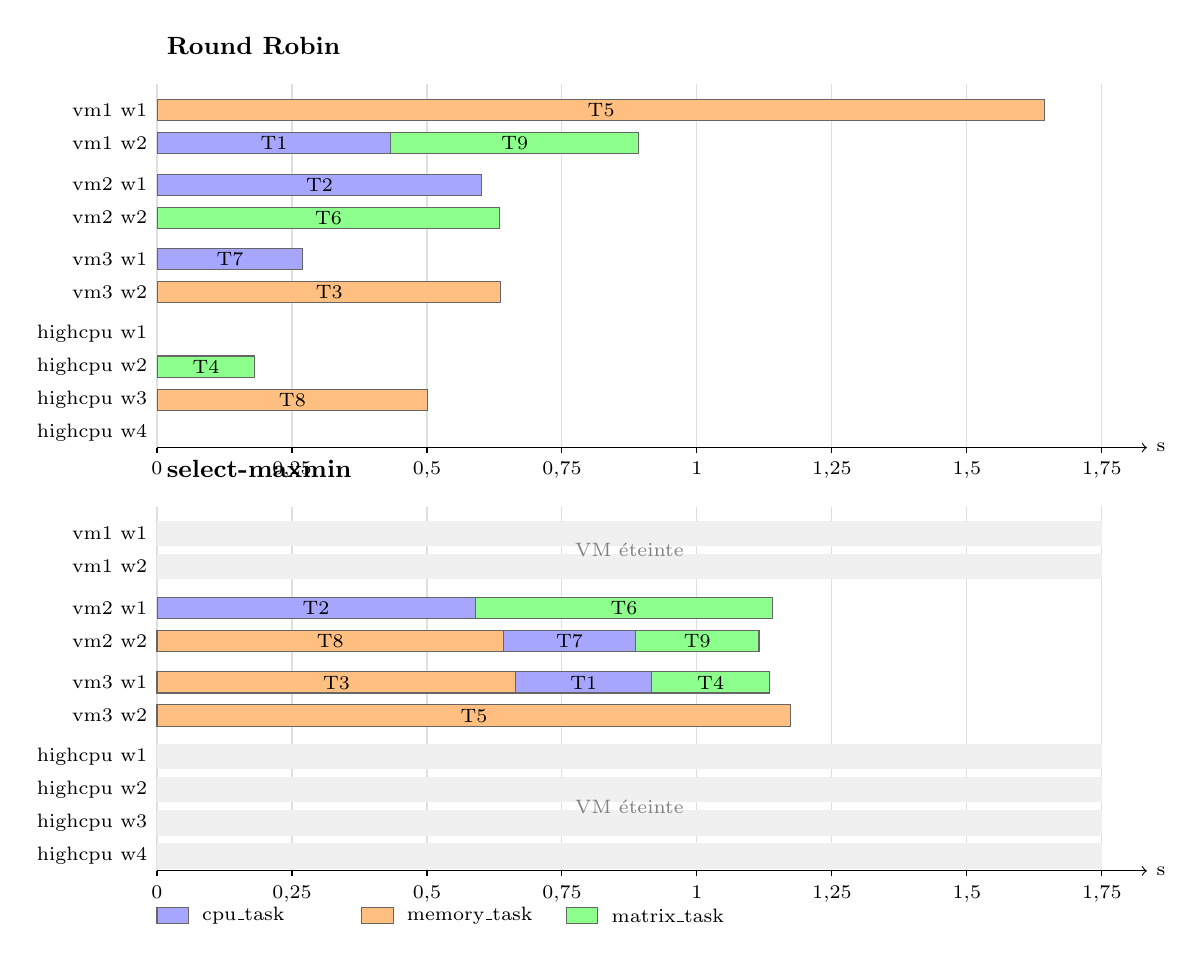
\begin{tikzpicture}[x=6.8571cm, y=0.42cm, font=\scriptsize]
  \node[anchor=south west, font=\small\bfseries] at (0,0.40) {Round Robin};
  \draw[gray!25] (0.0000,-11.20) -- (0.0000,-0.20);
  \draw[gray!25] (0.2500,-11.20) -- (0.2500,-0.20);
  \draw[gray!25] (0.5000,-11.20) -- (0.5000,-0.20);
  \draw[gray!25] (0.7500,-11.20) -- (0.7500,-0.20);
  \draw[gray!25] (1.0000,-11.20) -- (1.0000,-0.20);
  \draw[gray!25] (1.2500,-11.20) -- (1.2500,-0.20);
  \draw[gray!25] (1.5000,-11.20) -- (1.5000,-0.20);
  \draw[gray!25] (1.7500,-11.20) -- (1.7500,-0.20);
  \node[anchor=east] at (0,-1.00) {vm1 w1};
  \node[anchor=east] at (0,-2.00) {vm1 w2};
  \node[anchor=east] at (0,-3.25) {vm2 w1};
  \node[anchor=east] at (0,-4.25) {vm2 w2};
  \node[anchor=east] at (0,-5.50) {vm3 w1};
  \node[anchor=east] at (0,-6.50) {vm3 w2};
  \node[anchor=east] at (0,-7.75) {highcpu w1};
  \node[anchor=east] at (0,-8.75) {highcpu w2};
  \node[anchor=east] at (0,-9.75) {highcpu w3};
  \node[anchor=east] at (0,-10.75) {highcpu w4};
  \draw[fill=green!45, draw=black!60] (0.0002,-9.07) rectangle (0.1814,-8.43);
  \node at (0.0908,-8.75) {T4};
  \draw[fill=orange!50, draw=black!60] (0.0005,-10.07) rectangle (0.5011,-9.43);
  \node at (0.2508,-9.75) {T8};
  \draw[fill=blue!35, draw=black!60] (0.0008,-3.57) rectangle (0.6016,-2.93);
  \node at (0.3012,-3.25) {T2};
  \draw[fill=blue!35, draw=black!60] (0.0008,-2.32) rectangle (0.4330,-1.68);
  \node at (0.2169,-2.00) {T1};
  \draw[fill=orange!50, draw=black!60] (0.0008,-1.32) rectangle (1.6443,-0.68);
  \node at (0.8226,-1.00) {T5};
  \draw[fill=orange!50, draw=black!60] (0.0009,-6.82) rectangle (0.6370,-6.18);
  \node at (0.3190,-6.50) {T3};
  \draw[fill=green!45, draw=black!60] (0.0010,-4.57) rectangle (0.6341,-3.93);
  \node at (0.3176,-4.25) {T6};
  \draw[fill=blue!35, draw=black!60] (0.0012,-5.82) rectangle (0.2690,-5.18);
  \node at (0.1351,-5.50) {T7};
  \draw[fill=green!45, draw=black!60] (0.4331,-2.32) rectangle (0.8921,-1.68);
  \node at (0.6626,-2.00) {T9};
  \draw[->] (0,-11.20) -- (1.8333,-11.20) node[right] {s};
  \draw (0.0000,-11.20) -- (0.0000,-11.35) node[below] {0};
  \draw (0.2500,-11.20) -- (0.2500,-11.35) node[below] {0{,}25};
  \draw (0.5000,-11.20) -- (0.5000,-11.35) node[below] {0{,}5};
  \draw (0.7500,-11.20) -- (0.7500,-11.35) node[below] {0{,}75};
  \draw (1.0000,-11.20) -- (1.0000,-11.35) node[below] {1};
  \draw (1.2500,-11.20) -- (1.2500,-11.35) node[below] {1{,}25};
  \draw (1.5000,-11.20) -- (1.5000,-11.35) node[below] {1{,}5};
  \draw (1.7500,-11.20) -- (1.7500,-11.35) node[below] {1{,}75};
  \node[anchor=south west, font=\small\bfseries] at (0,-12.40) {select-maxmin};
  \draw[gray!25] (0.0000,-24.00) -- (0.0000,-13.00);
  \draw[gray!25] (0.2500,-24.00) -- (0.2500,-13.00);
  \draw[gray!25] (0.5000,-24.00) -- (0.5000,-13.00);
  \draw[gray!25] (0.7500,-24.00) -- (0.7500,-13.00);
  \draw[gray!25] (1.0000,-24.00) -- (1.0000,-13.00);
  \draw[gray!25] (1.2500,-24.00) -- (1.2500,-13.00);
  \draw[gray!25] (1.5000,-24.00) -- (1.5000,-13.00);
  \draw[gray!25] (1.7500,-24.00) -- (1.7500,-13.00);
  \node[anchor=east] at (0,-13.80) {vm1 w1};
  \fill[gray!12] (0,-14.18) rectangle (1.7500,-13.42);
  \node[anchor=east] at (0,-14.80) {vm1 w2};
  \fill[gray!12] (0,-15.18) rectangle (1.7500,-14.42);
  \node[gray] at (0.8750,-14.30) {VM éteinte};
  \node[anchor=east] at (0,-16.05) {vm2 w1};
  \node[anchor=east] at (0,-17.05) {vm2 w2};
  \node[anchor=east] at (0,-18.30) {vm3 w1};
  \node[anchor=east] at (0,-19.30) {vm3 w2};
  \node[anchor=east] at (0,-20.55) {highcpu w1};
  \fill[gray!12] (0,-20.93) rectangle (1.7500,-20.17);
  \node[anchor=east] at (0,-21.55) {highcpu w2};
  \fill[gray!12] (0,-21.93) rectangle (1.7500,-21.17);
  \node[anchor=east] at (0,-22.55) {highcpu w3};
  \fill[gray!12] (0,-22.93) rectangle (1.7500,-22.17);
  \node[anchor=east] at (0,-23.55) {highcpu w4};
  \fill[gray!12] (0,-23.93) rectangle (1.7500,-23.17);
  \node[gray] at (0.8750,-22.05) {VM éteinte};
  \draw[fill=orange!50, draw=black!60] (0.0001,-19.62) rectangle (1.1738,-18.98);
  \node at (0.5870,-19.30) {T5};
  \draw[fill=orange!50, draw=black!60] (0.0001,-17.37) rectangle (0.6416,-16.73);
  \node at (0.3209,-17.05) {T8};
  \draw[fill=orange!50, draw=black!60] (0.0001,-18.62) rectangle (0.6646,-17.98);
  \node at (0.3324,-18.30) {T3};
  \draw[fill=blue!35, draw=black!60] (0.0002,-16.37) rectangle (0.5891,-15.73);
  \node at (0.2946,-16.05) {T2};
  \draw[fill=green!45, draw=black!60] (0.5892,-16.37) rectangle (1.1406,-15.73);
  \node at (0.8649,-16.05) {T6};
  \draw[fill=blue!35, draw=black!60] (0.6417,-17.37) rectangle (0.8861,-16.73);
  \node at (0.7639,-17.05) {T7};
  \draw[fill=blue!35, draw=black!60] (0.6647,-18.62) rectangle (0.9160,-17.98);
  \node at (0.7903,-18.30) {T1};
  \draw[fill=green!45, draw=black!60] (0.8862,-17.37) rectangle (1.1150,-16.73);
  \node at (1.0006,-17.05) {T9};
  \draw[fill=green!45, draw=black!60] (0.9160,-18.62) rectangle (1.1348,-17.98);
  \node at (1.0254,-18.30) {T4};
  \draw[->] (0,-24.00) -- (1.8333,-24.00) node[right] {s};
  \draw (0.0000,-24.00) -- (0.0000,-24.15) node[below] {0};
  \draw (0.2500,-24.00) -- (0.2500,-24.15) node[below] {0{,}25};
  \draw (0.5000,-24.00) -- (0.5000,-24.15) node[below] {0{,}5};
  \draw (0.7500,-24.00) -- (0.7500,-24.15) node[below] {0{,}75};
  \draw (1.0000,-24.00) -- (1.0000,-24.15) node[below] {1};
  \draw (1.2500,-24.00) -- (1.2500,-24.15) node[below] {1{,}25};
  \draw (1.5000,-24.00) -- (1.5000,-24.15) node[below] {1{,}5};
  \draw (1.7500,-24.00) -- (1.7500,-24.15) node[below] {1{,}75};
  \draw[fill=blue!35, draw=black!60] (0.0000,-25.60) rectangle ++(0.0583,0.5);
  \node[anchor=west] at (0.0656,-25.35) {cpu\_task};
  \draw[fill=orange!50, draw=black!60] (0.3792,-25.60) rectangle ++(0.0583,0.5);
  \node[anchor=west] at (0.4448,-25.35) {memory\_task};
  \draw[fill=green!45, draw=black!60] (0.7583,-25.60) rectangle ++(0.0583,0.5);
  \node[anchor=west] at (0.8240,-25.35) {matrix\_task};
\end{tikzpicture}

\caption{Diagramme temporel de la première exécution de chaque
algorithme sur 9 tâches : une ligne par worker, une barre par tâche (début et fin
relevés par l'orchestrateur). Round Robin allume les 4 VM et laisse la moitié des
workers de highcpu inactifs ; \sel{} n'allume que vm2 et vm3 et occupe leurs deux
workers en parallèle pendant tout le lot.}
\label{fig:gantt}
\end{figure}

\paragraph{Lecture.}
\begin{itemize}
  \item \textbf{Sur 9 et 500 tâches, \sel{} obtient le meilleur score mesuré},
        devant les cinq heuristiques et l'allocation manuelle : il éteint des VM,
        ce que les autres ne font pas.
  \item Sur 500 tâches, \textbf{cette victoire vient entièrement du coût}
        ($-28\,\%$). Avec 3 exécutions et des écarts-types de 9 à 20~s, les écarts
        de makespan ne sont pas significatifs : son lot est même plus long, car
        vm3 a été bridée pendant 2 de ses 3 exécutions.
  \item \textbf{Sur 2000 tâches, \sel{} est à égalité avec Max-Min, MCT et
        Min-Min} (écarts inférieurs à 1\,\%, dans le bruit de mesure). Il garde
        les 4 VM : son allocation est alors exactement celle de Max-Min.
  \item \textbf{La contrainte de délai est aussi respectée en réel} par \sel{} sur
        tous les lots (au plus 1,23, sur 9 tâches en session 1). Seul MET la
        dépasse, sur 2000 tâches (1,26), ce que le modèle avait prévu. Sur
        500 tâches, le modèle prévoyait aussi MET non admissible (51,9~s pour
        une limite de 50,6~s), mais il passe en réel (1,21) : RR, ralenti par
        vm3 dans cette session, a relâché la contrainte. C'est la limite d'une
        échéance relative à RR (section~\ref{sec:limites}).
  \item \textbf{Le classement mesuré suit globalement le classement prédit},
        sauf Min-Min sur 9 tâches : prédit avec le pire score, il est en réalité
        le plus rapide (section~\ref{sec:limites}).
\end{itemize}

\subsection{Précision du modèle}

\begin{table}[H]
\centering\small
\begin{tabular}{llr@{\hspace{1.2em}}ccc@{\hspace{1.2em}}ccc}
\toprule
 & & \textbf{Prédit} & \multicolumn{3}{c}{\textbf{Mesuré (s)}} & \multicolumn{3}{c}{\textbf{Mesuré / prédit}} \\
\cmidrule(lr){4-6}\cmidrule(lr){7-9}
\textbf{Lot} & \textbf{Session} & \textbf{(s)} & r1 & r2 & r3 & r1 & r2 & r3 \\
\midrule
9 tâches    & 1 & 1,27  & 1,54  & 1,23  & 1,36  & 1,22 & 0,97 & 1,08 \\
            & 2 & 1,27  & 1,17  & 1,16  & 1,26  & 0,93 & 0,91 & 0,99 \\
\midrule
500 tâches  & 1 & 39,7  & 41,5  & 51,4$^{b}$  & 74,5$^{b}$  & \textbf{1,05} & 1,30 & 1,88 \\
            & 2 & 39,7  & 70,8$^{b}$  & 71,0$^{b}$  & 54,8$^{b}$  & 1,78 & 1,79 & 1,38 \\
\midrule
2000 tâches & 1 & 136,1 & 256,8$^{b}$ & 254,6$^{b}$ & 251,3$^{b}$ & 1,89 & 1,87 & 1,85 \\
            & 2 & 136,1 & 255,5$^{b}$ & 253,7$^{b}$ & 256,2$^{b}$ & 1,88 & 1,86 & 1,88 \\
            & 3 & 136,1 & 263,9$^{b}$ & 262,2$^{b}$ & 148,1 & 1,94 & 1,93 & \textbf{1,09} \\
            & 4$^{\ddagger}$ & 136,1 & 161,0$^{b}$ & 165,7$^{b}$ & 161,3$^{b}$ & 1,18 & 1,22 & 1,19 \\
\bottomrule
\end{tabular}
\caption{Makespan de \sel{} : prédit par le modèle et mesuré sur GCP, pour
chacune des 24 exécutions. $^{b}$ vm3 bridée pendant l'exécution (plus de 1,3 fois
plus lente que vm2 pour la même charge). $^{\ddagger}$ VM démarrées sur processeur AMD EPYC 7B12, contre Intel Xeon @ 2.20GHz dans toutes les autres sessions (modèle relevé par l'orchestrateur).
Sources : \code{results/exp\_real/} et \code{results/exp\_real\_all/}
(\code{predicted.csv}, \code{runs.csv}, \code{*\_vms.csv}).}
\label{tab:precision_select}
\end{table}

\paragraph{Lecture.}
\begin{itemize}
  \item \textbf{Quand aucune VM n'est bridée, le modèle est précis} : le rapport
        mesuré/prédit va de 0,91 à 1,22 (9 tâches, 500 tâches r1, 2000 tâches
        session 3 r3), soit une erreur d'environ $\pm 10$ à 20\,\%.
  \item \textbf{Quand vm3 est bridée, le lot dure jusqu'à 1,9 fois plus longtemps
        que prévu} : le makespan est fixé par la VM la plus lente, et le modèle ne
        peut pas prévoir ce bridage.
  \item Sur 9 tâches, chaque VM n'exécute que quelques tâches, en moins de 2~s :
        aucune n'a le temps d'être bridée.
  \item En session~4 des 2000 tâches, le rapport reste à 1,2 malgré le bridage de
        vm3, parce que les VM tournaient sur processeur AMD, plus rapide que les
        Intel sur lesquels le modèle a été calibré : les deux effets se compensent
        en partie.
\end{itemize}

\paragraph{D'où vient l'erreur ?} Pour le savoir, nous avons comparé l'heure de fin
mesurée et prédite de chaque VM séparément (session 1).

\begin{table}[H]
\centering\small
\begin{tabular}{llcccc}
\toprule
\textbf{Lot} & \textbf{Algorithme} & \textbf{highcpu} & \textbf{vm1} & \textbf{vm2} & \textbf{vm3} \\
\midrule
9    & RR    & 0,72 & 0,89 & 1,01 & 0,93 \\
9    & \sel  & —    & —    & 0,92 & 1,12 \\
500  & RR    & 1,02 & 1,09 & 0,92 & 0,99 \\
500  & \sel  & 1,05 & —    & 0,95 & 1,30 \\
2000 & RR    & 1,02 & 1,09 & 1,15 & \textbf{1,91} \\
2000 & \sel  & 1,05 & 1,15 & 0,96 & \textbf{1,87} \\
\bottomrule
\end{tabular}
\caption{Heure de fin mesurée / prédite pour chaque VM (session~1, médiane des
3 exécutions).}
\label{tab:precision}
\end{table}

Sur 500 et 2000 tâches, hors vm3, le modèle se trompe de $-8$ à $+15\,\%$
(highcpu : $+2$ à $+5\,\%$) ; sur 9 tâches, les écarts sont plus grands (2 ou
3 tâches par VM). vm3 a fortement ralenti sur les lots longs : 1,7 à 1,9 fois
plus lente que prévu sur 2000 tâches, quel que soit l'algorithme. Or le makespan
est fixé par la VM la plus lente : \textbf{une seule VM ralentie suffit à fausser
la prédiction du lot entier} (section~\ref{sec:vm3}).

\subsection{Investigation : le ralentissement des e2-medium}
\label{sec:vm3}

Sur les lots longs, le makespan était souvent bien supérieur à la prédiction.
Pour comprendre pourquoi, nous avons regardé le temps de travail de chaque VM
séparément. Avec \sel{}, l'allocation de 2000 tâches est la même à chaque
session : 388 tâches sur vm2 et 398 sur vm3, deux e2-medium. Elles devraient donc
finir presque en même temps.

\begin{table}[H]
\centering\small
\begin{tabular}{llcc}
\toprule
\textbf{Session} & \textbf{vm3} & \textbf{vm2 (s) : r1 / r2 / r3} & \textbf{vm3 (s) : r1 / r2 / r3} \\
\midrule
1 & d'origine & 130 / 130 / 132 & 257 / 255 / 251 \\
2 & d'origine & 165 / 132 / 132 & 256 / 254 / 256 \\
3 & recréée   & 172 / 131 / 131 & 264 / 262 / 148 \\
4$^{\ddagger}$ & recréée &  87 /  92 /  88 & 161 / 166 / 161 \\
\bottomrule
\end{tabular}
\caption{Temps de travail de vm2 et vm3 sur les 12 exécutions de \sel{} sur
2000 tâches (\mesure{}). Même type de VM, même charge à 3\,\% près.
$^{\ddagger}$ VM démarrées sur processeur AMD EPYC 7B12, contre Intel Xeon @ 2.20GHz dans toutes les autres sessions (modèle relevé par l'orchestrateur).}
\label{tab:vm2vm3}
\end{table}

Les sessions 2 et 3 ont été lancées pour étudier vm3, pas pour comparer les
algorithmes : elles ne figurent donc pas dans les tableaux de synthèse. Leurs
exécutions de RR (241 à 348~s) sont dans \code{results/exp\_real/tasks\_2000\_session2/}
et \code{tasks\_2000\_vm3neuve/} ; la dernière de la session 3 est exclue (surcoût
SSH multiplié par 5 sur les 4 VM à la fois, incident côté machine de contrôle).
Sur ces 5 paires valides, \sel{} est plus rapide que RR dans 3. Les 2 autres sont
les premières exécutions de chaque session : vm3 n'était pas encore bridée pendant
l'exécution de RR, mais l'était pendant celle de \sel{}. En moyenne sur chaque
session, \sel{} reste plus rapide : $-17\,\%$ en session~2 et $-11\,\%$ en
session~3 (sur les paires valides).

\paragraph{Lecture.}
\begin{itemize}
  \item \textbf{vm3 met presque deux fois plus de temps que vm2} dans 11 exécutions
        sur 12. Le temps de calcul mesuré par les workloads eux-mêmes double : c'est
        le processeur qui est ralenti, pas le réseau.
  \item \textbf{Ce n'est pas une machine défectueuse} : nous avons supprimé puis
        recréé vm3, qui s'est probablement retrouvée sur un autre serveur
        physique. Le ralentissement est resté le même (sessions 3 et 4).
  \item vm2 n'a connu que deux épisodes légèrement lents (165 et 172~s), tous deux
        en début de session.
\end{itemize}

\paragraph{Explication.} La documentation de
GCP\footnote{\url{https://cloud.google.com/compute/docs/general-purpose-machines\#cpu-bursting}}
indique que chacun des 2~vCPU d'une e2-medium n'a droit qu'à 50\,\% du temps
processeur, soit l'équivalent d'un seul vCPU. Au-delà, la VM fonctionne par
\emph{rafales} limitées dans le temps. Privée de rafale, elle tourne donc environ
deux fois moins vite, ce que nous mesurons. Avec Round Robin, vm3 n'était
d'ailleurs normale qu'à la \emph{première} exécution de chaque session, puis
ralentissait, ce qui va dans le sens d'une réserve de rafale qui s'épuise. Ce
mécanisme n'explique pas pourquoi vm3 est bridée et pas vm2 : cela dépend
probablement de l'occupation du serveur physique, que nous ne contrôlons pas.
highcpu a été stable dans toutes nos mesures. vm1 (sans cœur partagé) a ralenti
lors d'une session (47 à 66~s au lieu de $\approx 31$~s sur 500 tâches).

\paragraph{Conséquence : nous dépendons de Google.} Sur un lot long, le makespan
est fixé par la VM la plus lente, quel que soit l'algorithme. Or la vitesse réelle
d'une VM dépend de deux choses que le client ne voit pas et ne choisit pas :
\begin{itemize}
  \item \textbf{le serveur physique attribué} : GCP choisit lui-même le processeur
        à chaque démarrage d'une VM e2. Nous l'avons constaté : toutes nos sessions
        ont tourné sur Intel Xeon @ 2.20GHz, sauf la session~4 des 2000 tâches, sur
        AMD EPYC 7B12, où les VM non bridées étaient environ 35\,\% plus rapides
        (highcpu : 92~s au lieu de 143~s pour les mêmes 817 tâches).
        L'orchestrateur l'a enregistré car il relève le modèle de processeur à
        chaque exécution ;
  \item \textbf{l'activité des autres clients sur ce serveur} : une e2-medium ne
        dépasse sa part garantie que si le serveur a du processeur libre. Deux VM
        identiques peuvent donc tourner à des vitesses très différentes, comme vm2
        et vm3. Nous ne pouvons pas le prouver directement (le serveur physique
        n'est pas visible), mais c'est l'explication la plus cohérente avec nos
        mesures.
\end{itemize}
Quand une VM est bridée, toute prédiction faite à l'avance est donc fausse d'un
facteur proche de 2. Ce n'est pas un défaut du modèle qu'un meilleur calibrage
corrigerait : c'est une incertitude propre au cloud mutualisé, qu'un scheduler
doit accepter et gérer. C'est la principale limite de notre approche
(section~\ref{sec:limites}).
